\section{The \ac{CLEAVE} framework}\label{sec:approach}

In this section, we detail our \ac{CLEAVE} framework for the performance evaluation of \aclp{NCS}, with an emphasis on edge deployments.
Our design follows a virtualized emulation approach; providing a framework for the real-time \emph{emulation} of physical control systems and the easy implementation of softwarized controllers interacting with \emph{real} networks.
\ac{CLEAVE} is thus, a platform with an easy-to-use \ac{API} on which a multitude of \ac{NCS} types can be emulated.
This allows for great flexibility, as the core components of the \ac{NCS} can be switched out while maintaining the realism of the network, the most complex and limiting component of edge \acp{NCS}.

The framework is distributed as \emph{free and open-source} software through the \emph{GitHub} organization of the \emph{KTH ExPECA} research group\footnote{\url{https://github.com/KTH-EXPECA/CLEAVE}}.
We also plan to provide a library of \ac{NCS} implementations, making the tool even more accessible.

\subsection{Design and Implementation}

\cref{fig:cleave:ncs:struct} shows an overview of the conceptual structure and operation of \ac{CLEAVE}.
The \emph{State} implements the discrete-time behavior of the Plant.
At the beginning of each time-step, actuated variables in the \emph{State} are updated with values obtained from the \emph{Actuator} objects.
Conversely, at the end of each time-step, sensed variables are sampled and used to update values associated with \emph{Sensor} objects.
These values are processed at the \emph{Sensors} (e.g.\ to add noise) before being sent over the network to the \emph{Controller}.
The \emph{Controller} calculates actuation values and updates the \emph{Actuators} over the network.
Finally, the \emph{Actuators} process the actuation values and hold the results until they are read at the next time-step.

Implementation-wise, \ac{CLEAVE} is built on top of the well-established and stable \emph{Twisted}\footnote{\url{https://twistedmatrix.com}} asynchronous programming and networking framework.
The aforementioned core components (\emph{State}, \emph{Controller}, \emph{Sensors}, and \emph{Actuators}) are provided as \acp{ABC} with core functionality that users must extend for their specific use cases and \acp{NCS}.
The framework makes no assumptions about the inner workings of the user implementations of these classes other than the interfaces they expose.
Users are therefore free to implement arbitrarily complex functionality in these components.
On the other hand, \ac{CLEAVE} handles network communication and metric collection autonomously; users only need to select the desired transport protocol (we do however provide an \ac{API} for extending the available transports).

Below we present a brief overview of the design and implementation of the core components.

%\begin{description}[style=nextline]
%\begin{itemize}
\textbf{State Base Class}:
\ac{ABC} with an abstract method
\mintinline{python}{advance()} which must be extended with the implementation of discrete-time emulation of the plant.
The \mintinline{python}{advance()} method is called by the framework periodically according to the configured emulation update rate, and should perform a single time-step of the discrete-time emulation.
Two optionally extensible methods, \mintinline{python}{initialize()} and \mintinline{python}{shutdown()} are provided to implement single-fire set-up and tear-down procedures.

    % This class also provides functionality for the automatic tracking and updating of sensed and actuated values.
    % This is handled through special auxiliary classes, \emph{SensorVariable} and \emph{ActuatorVariable}, which when instantiated and assigned to an attribute of the \emph{State} allow the framework to track and modify them.

\textbf{Controller Base Class}:
Defines a single abstract method \mintinline{python}{process()}, taking a mapping of names to values corresponding to the sensed variables of the \emph{State}, and returning a similar mapping corresponding to the actuated variables.
This method is called by \ac{CLEAVE} in an event-based manner whenever samples are received from the plant side; however, we intend to extend this to time-interval-based approaches.

\textbf{Sensor Base Class}:
Implements processing of monitored stated variables before sending them over the network to the \emph{Controller}.
This base class must be initialized with a property name (corresponding to the monitored \emph{State} attribute) and a sampling rate in \si{\hertz}, and provides an abstract method \mintinline{python}{process_sample()} which must be extended with an implementation of the processing performed on each sample.

\textbf{Actuator Base Class}:
Performs the processing of actuation values obtained over the network from the \emph{Controller}.
It is initialized with a property name corresponding to the name of the actuated \emph{State} attribute, and provides two abstract methods which must be implemented by extending classes:
\begin{enumerate*}[itemjoin={{; }}, itemjoin*={{; and }}]
\item \mintinline{python}{set_value()}, called by the framework whenever a new value for the corresponding actuated attribute is received
\item \mintinline{python}{get_actuation()}, called on every time-step and must return a value to apply to the actuated attribute.
\end{enumerate*}
%\end{itemize}
%\end{description}


\subsection{Configuring and Executing \iac{NCS}}

Once the core components for the emulation have been defined and implemented, they need to be registered with the framework.
This is done through Python scripts which define a number of required (and some optional) top-level variables, corresponding to emulation parameters such as the \emph{State}, \emph{Controller}, \emph{Sensor}, and \emph{Actuator} subclasses to use; the emulation update rate; the controller-side host and address; data output directories; \emph{et cetera}.
These Python configuration files are then provided as arguments to the \texttt{cleave} command line provided by the framework.
\ac{CLEAVE} imports and parses them, and then sets up and executes the emulation.

Although the core design of \ac{CLEAVE} follows a single-loop approach, multi-loop scenarios can be easily implemented through the combination of multiple \ac{CLEAVE} instances.
The framework doesn't assume the individual components other than the signatures of methods on the base classes that must be extended and implemented.
Combined with the Python emulation configuration scripts, this makes development of more complex scenarios merely a matter of implementing the desired functionality within the framework itself.

\subsection{Current Implementations}

\begin{figure}
    \centering
    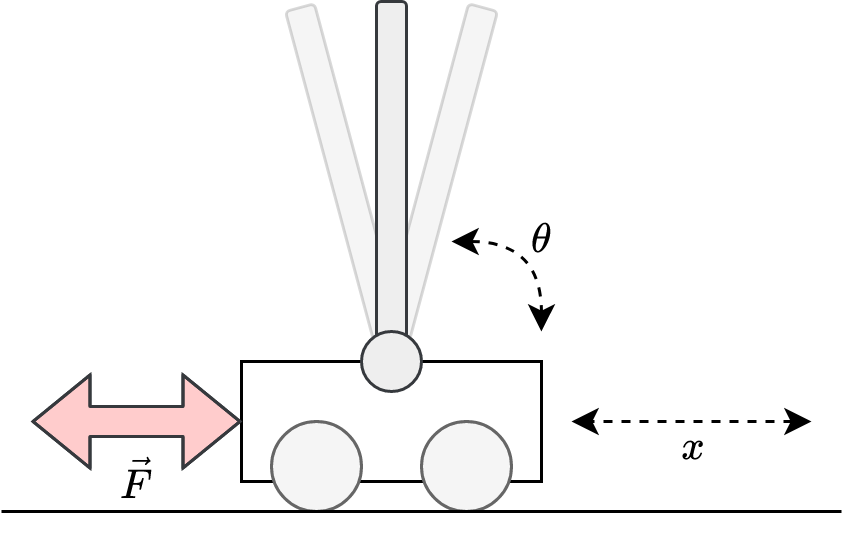
\includegraphics[width=.7\columnwidth]{images/inverted_pendulum.png}
    \caption{
        The 2D inverted pendulum system.
    }\label{fig:invpend}
\end{figure}

For the purpose of this work, we have used \ac{CLEAVE} to implement an emulated \emph{inverted pendulum} control loop (see \cref{fig:invpend}), the goal of which is to balance the vertically free-swinging pendulum by applying horizontal forces on the cart.
We have chosen this system as an initial benchmark for its relative simplicity as well as prevalence in the field of automatic control as one of the fundamental examples of linear control.
However, as mentioned above, we eventually plan to build an open library of emulated control loops.  

The inverted pendulum plant \emph{State} is implemented as a real-time discrete-time physical emulation using CLEAVE's API and a 2D physics library\footnote{Pymunk: \url{http://www.pymunk.org/en/latest/}}, updated at a constant \SI{120}{\hertz} (this value is configurable; in this case it corresponds to the maximum achievable stable rate on the clients).
\emph{Sensors} for the angle, position, angular velocity, and velocity of the \emph{State}, and an \emph{Actuator} for the horizontal force applied to the cart are implemented as ``perfect'', i.e.\ values are returned as-is, without any added noise.
For the controller side, a proportional-differential strategy is implemented using the framework \emph{Controller} API and the \emph{NumPy} numeric computation library\footnote{NumPy: \url{https://numpy.org/}}.
Plant and controller are then packaged into containers, for ease of orchestration and reparametrization, and to mimic real-world deployment.
